\chapter{CritiqueKit: Interactive Guidance Techniques for Improving Creative Feedback}
\label{chapter:critiquekit}
\begin{quote}
Good feedback is critical to creativity and learning, yet rare. Many people do not know how to actually provide effective feedback. There is increasing demand for quality feedback – and thus feedback givers – in learning and professional settings. This chapter contributes empirical evidence that two interactive techniques – reusable suggestions and adaptive guidance – can improve feedback on creative work. We present these techniques embodied in the \textit{CritiqueKit} system to help reviewers give specific, actionable, and justified feedback. Two real-world deployment studies and two controlled experiments with CritiqueKit found that adaptively-presented suggestions improve the quality of feedback from novice reviewers. Reviewers also reported that suggestions and guidance helped them describe their thoughts and reminded them to provide effective feedback.
\end{quote}

\section{Introduction: Feedback's Hidden Potential}
Feedback is one of the most powerful influences on learning and achievement [14]. Both giving and receiving formative feedback encourage self-reflection and critical thinking on one's work [24,31], especially in creative and open-ended domains such as design and writing [14,35]. The growing scale of many educational and professional settings increases both the importance and difficulty of providing sufficiently descriptive and personalized feedback. Good feedback can be hard to generate, and people are not consistently skilled in doing so [22,46]. Feedback is often too short, vague, and not actionable [20,40,45]. Even experienced reviewers don't always recognize when they are providing poor feedback or why it is ineffective [40].

This paper contributes two interactive techniques that improve feedback, their embodiment in the CritiqueKit system, and their evaluation through two deployments and two experiments.

\textbf{Interactive guidance of feedback characteristics.} CritiqueKit features a guidance panel with checkboxes that update as the reviewer gives feedback. A text classifier categorizes feedback as Specific, Actionable, and/or Justified as the reviewer types, providing them with an ambient awareness of their feedback quality and guiding them to improve their feedback. 

\textbf{Suggesting prior feedback for reuse.} CritiqueKit enables reviewers to reuse expert feedback, reducing experts' labor by scaling their feedback to similar work. These suggestions update and adapt based on the feedback's categorization to give reviewers targeted ideas for how to improve their comment and provide inspiration. 

Two deployment studies and two controlled experiments investigated the efficacy of these interactive techniques on the quality and characteristics of feedback. The first deployment examined how experienced reviewers (teaching assistants) reuse feedback in an undergraduate course. The second deployment examined how undergraduate students reuse feedback. The first experiment examined the impact of statically presented suggestions and interactive guidance on novice feedback. Finally, the second experiment examined the efficacy of adaptively updating suggestions in tandem with interactive guidance on novice feedback. We found that adaptively-presented suggestions improved feedback quality (\autoref{fig:critiquekit_exp2}). Reviewers found suggestions useful for inspiration, and the interactive guidance reminded them to ensure their comments met the criteria for effective feedback. This work provides evidence that interactive techniques such as suggestions and guidance can effectively scaffold the feedback process (See \autoref{table:critiquekit_all_results} for details).

\begin{table}
\centering
  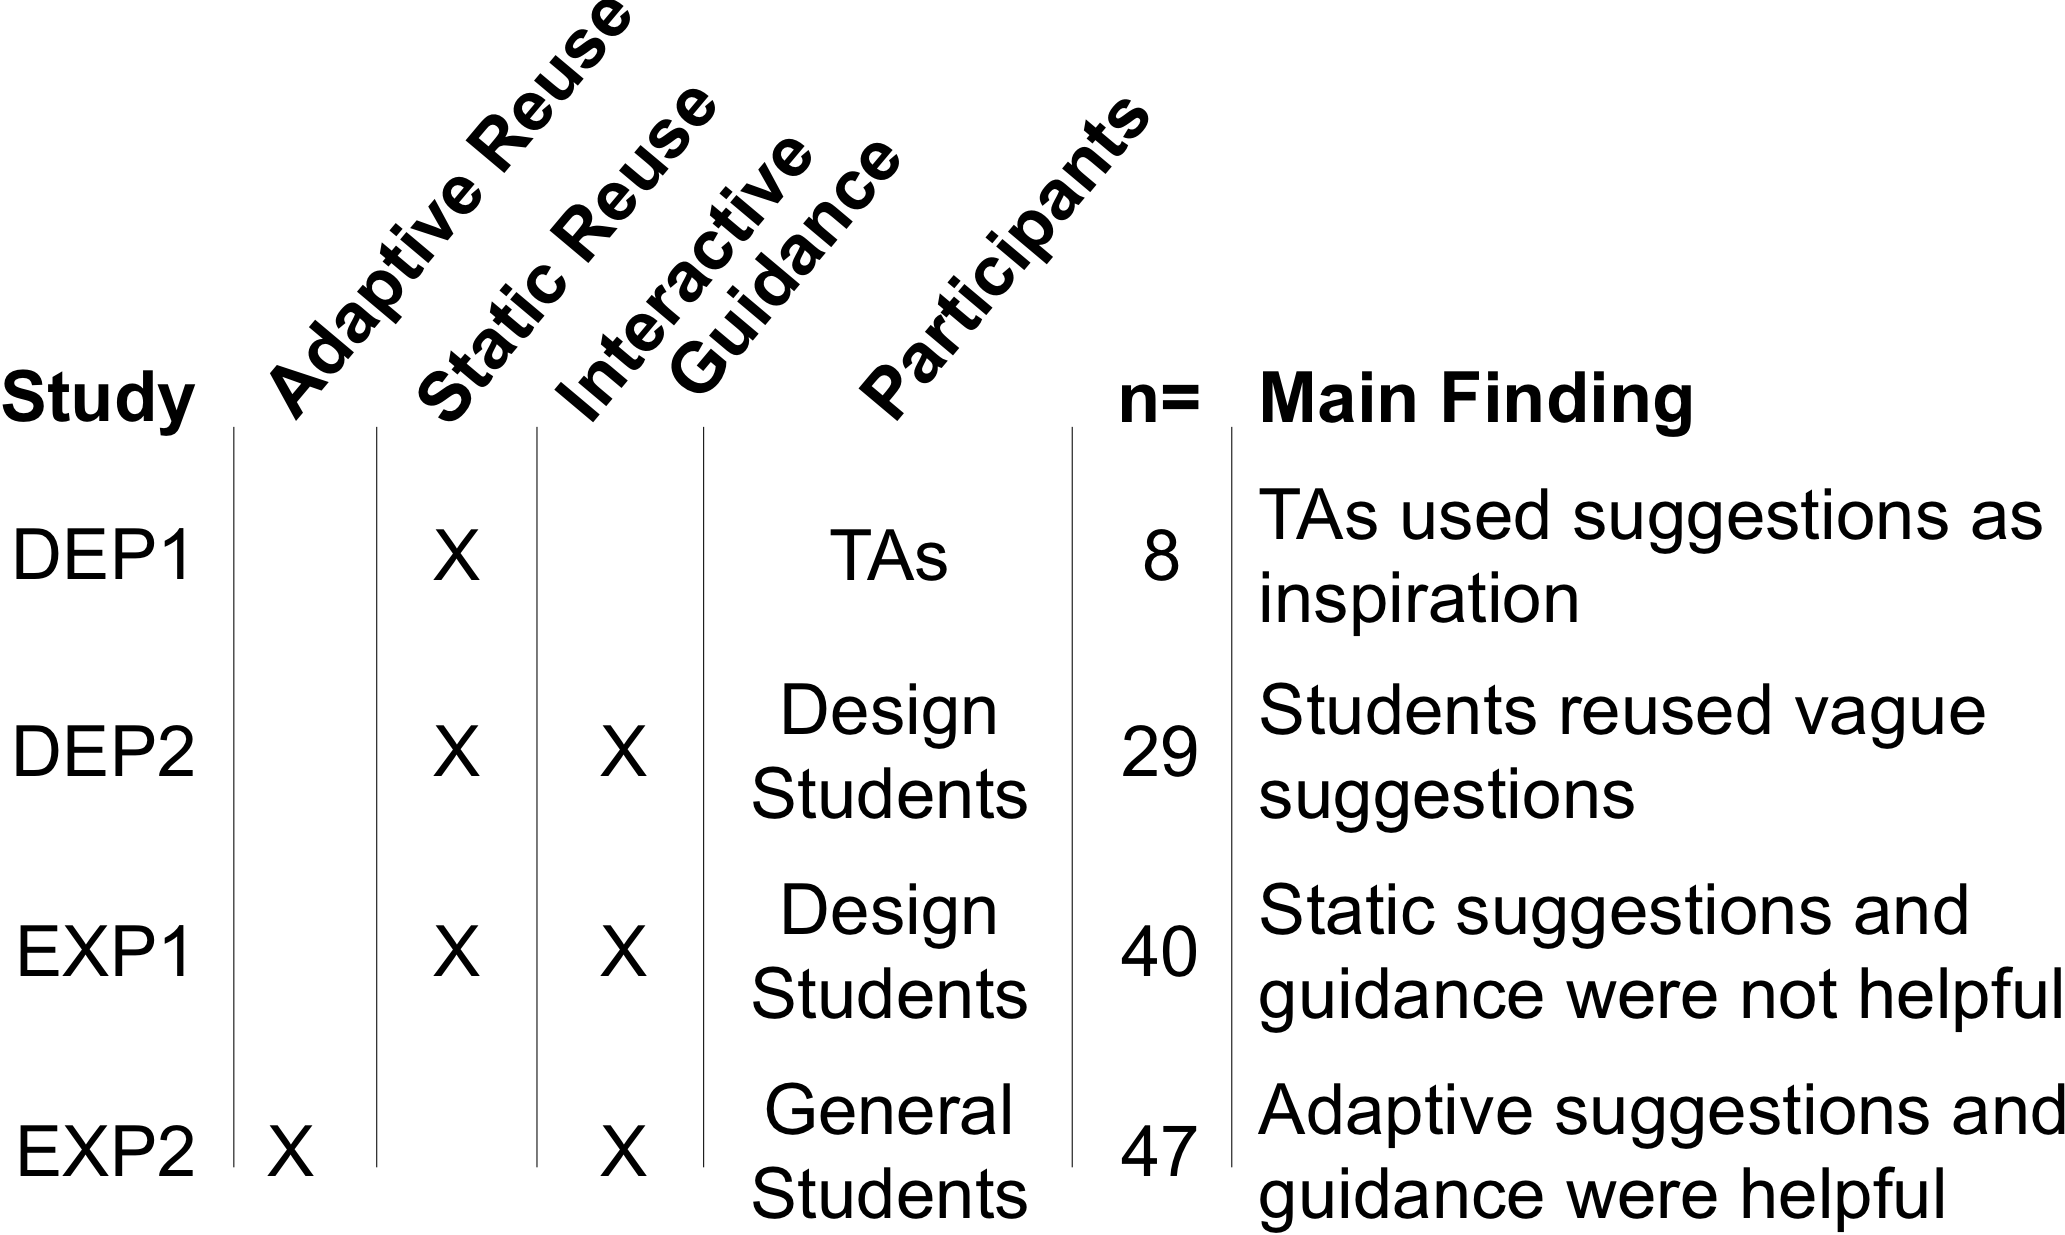
\includegraphics[width=0.6\textwidth]{critiquekit/figures/table1.png}
  \caption{Two deployments (DEP) and two between-subjects experiments (EXP) examined the efficacy of feedback reuse and interactive guidance. We found that interactive suggestions and guidance were most helpful for improving feedback.}~\label{table:critiquekit_all_results}
\end{table}

\section{Related Work}
\subsection{Good Feedback is Actionable, yet Rare}
Rapid iteration is critical to the success of creative projects, from essays, to visual design, to buildings \cite{Dow2010, Sadler1989}. Receiving feedback early on is important for learners to test alternatives and course-correct \cite{Dow2010, Tohidi2006}. Effective feedback is especially important in educational settings where novices are learning new skills and developing expertise. However, giving effective feedback is rarely taught \cite{Nicol2006}. As physical and digital classrooms increase in size, the demand for feedback outgrows the ability to adopt the ideal learning model of one-to-one feedback \cite{Bloom1984}. Instead, a one-to-many approach is utilized, where an expert provides feedback for multiple learners. Although learners most value expert feedback \cite{Gielen2010, Yang2006}, the one-to-many approach is highly demanding on experts, and specific, actionable feedback for individuals becomes increasingly rare. 

In general, effective feedback is specific, actionable, and justified. Specific feedback is direct and related to a particular part of the work rather than vaguely referent \cite{Krause2017, Sadler1989, Yuan2016}. Specific positive feedback also highlights strengths of the work and provides encouragement, so the recipient can tell they are on a good path \cite{Kelley2013, Tseng2007, Yuan2016}. Actionable feedback is important because it offers the learner a concrete step forward \cite{Sadler1989, Sommers1982, Tseng2007, Yuan2016}. Simply pointing out a problem is not sufficient to help one improve \cite{Ramaprasad1983, Sadler1989, Sommers1982, Tohidi2006}. Actionable feedback is often most helpful early in a project \cite{Cho2006, Tseng2007, Yuan2016} because it may help people self-reflect and self-evaluate their work \cite{Gibbs}, prompting more revisions for improvement \cite{Dow2012, Topping1998}. Lastly, justification is an important characteristic of feedback \cite{Krause2017, Narciss2006, Yuan2016}, but is arguably one of the hardest to understand or recognize \cite{Gielen2010}. Justified feedback contains an explanation or reason for a suggested change, which helps the learner understand why the feedback was given.

\subsection{Rubrics \& Examples Usefully Focus Feedback}
Rubrics \cite{Andrade2005, Yuan2016} and comparative examples \cite{Krause2017} are effective in structuring feedback because they beneficially encourage attention to deep and diverse criteria. Novices otherwise tend to focus on the first thing they notice, often surface-level details \cite{Greenberg2015, Hicks2016, Kulkarni2015, Yuan2016}. Viewing examples of past designs can lead to greater creativity and insights \cite{Kulkarni2014, Marsh1996}; thus, showing examples of good feedback may spark ideas reviewers would not have otherwise considered \cite{Greenberg2015, Kulkarni2013, Luther2015}. Also, adaptive examples curated to match design features are more helpful than random examples in improving creative work \cite{Lee2010}. 

Rubrics and other scaffolds require significant upfront manual work by experts who must carefully design a comprehensive rubric, curate a thorough set of examples, or decide how else to structure the feedback process. This chapter investigates leveraging existing feedback to dynamically create rubric criteria. We hypothesize that showing reviewers previously-provided feedback can guide their attention to important aspects of the design. 
\subsection{Is Feedback too Context-specific for Practical Reuse?}
Schön persuasively argues that effective feedback should be context-specific and expert-generated \cite{Schon1983}. He offers a vignette from architecture where the teacher suggests an alternative building to the student as an example of situated wisdom and its transfer. If Schön is right that this exchange requires both wisdom and context, does that mean that feedback reuse is infeasible? Within a given setting, project, or genre, common issues recur. Hewing to the principle of recognition over recall, we hypothesize that suggestions and guidance can increase novices' participation in context-specific exchanges. 

\subsection{Prior Systems \& Approaches for Scaling Feedback}
Existing approaches for scaling personalized feedback include clustering by similarity (\textit{e.g.}, for writing \cite{Brooks2014} and programming \cite{Glassman2015, Head2017}). Gradescope \cite{Singh2017} and Turnitin \cite{Turnitin} allow graders to create reusable rubric items and comments to address common issues and apply them across multiple assignments. Gradescope binds rubric items to scores, which emphasizes grades rather than improvement. 

Other methods include automating the reuse of the solutions of previous learners. These methods work best when correct and incorrect solutions are clearly distinct, such as in programming \cite{Glassman2016Learnersourcing, Hartmann2010} and logical deductions \cite{Fast2013}. Automated methods have also found success with the formal aspects of more open-ended domains such as writing \cite{Brooks2014, Roscoe2014}.  However, assessing the quality and effectiveness of creative work – the strength of a design, the power of a poem – is intrinsically abstract and subjective and lies beyond current automated analysis techniques. Also, little automated analysis exists for media other than text. For domains like design, human-in-the-loop analysis will remain important for quite some time. 

\subsection{Automatically Detecting Feedback Characteristics}
Although feedback is often specific and contextual \cite{Schon1983}, general characteristics can be automatically detected and used to help reviewers improve their feedback. For example, PeerStudio \cite{Kulkarni2015} detects when comments can be improved based on the length of the comment and the number of relevant words. Data mining and natural-language processing techniques can also automatically detect whether a comment is actionable or not, and prompt the reviewer to include a solution \cite{Nguyen2016, Xiong2012}. Krause \textit{et al.} use a natural-language processing model to detect linguistic characteristics of feedback and suggest examples to reviewers to help them improve their comment \cite{Krause2017}. These methods require a reviewer to first submit their comment so it can be analyzed, and then improve their comment after submission.

\section{CritiqueKit: Interactively Guiding Feedback}
Based on these methods and insights, CritiqueKit (\autoref{fig:critiquekit_interface}) categorizes feedback and provides prompts and suggestions to reviewers. It differs from prior work by providing feedback to reviewers as they type rather than after they submit. We hypothesize that this ambient feedback with suggestions may provide a just-in-time scaffold that changes how reviewers' thoughts crystallize, yielding feedback that is more specific, actionable, and/or justified. 

\begin{figure}[b!]
\centering
  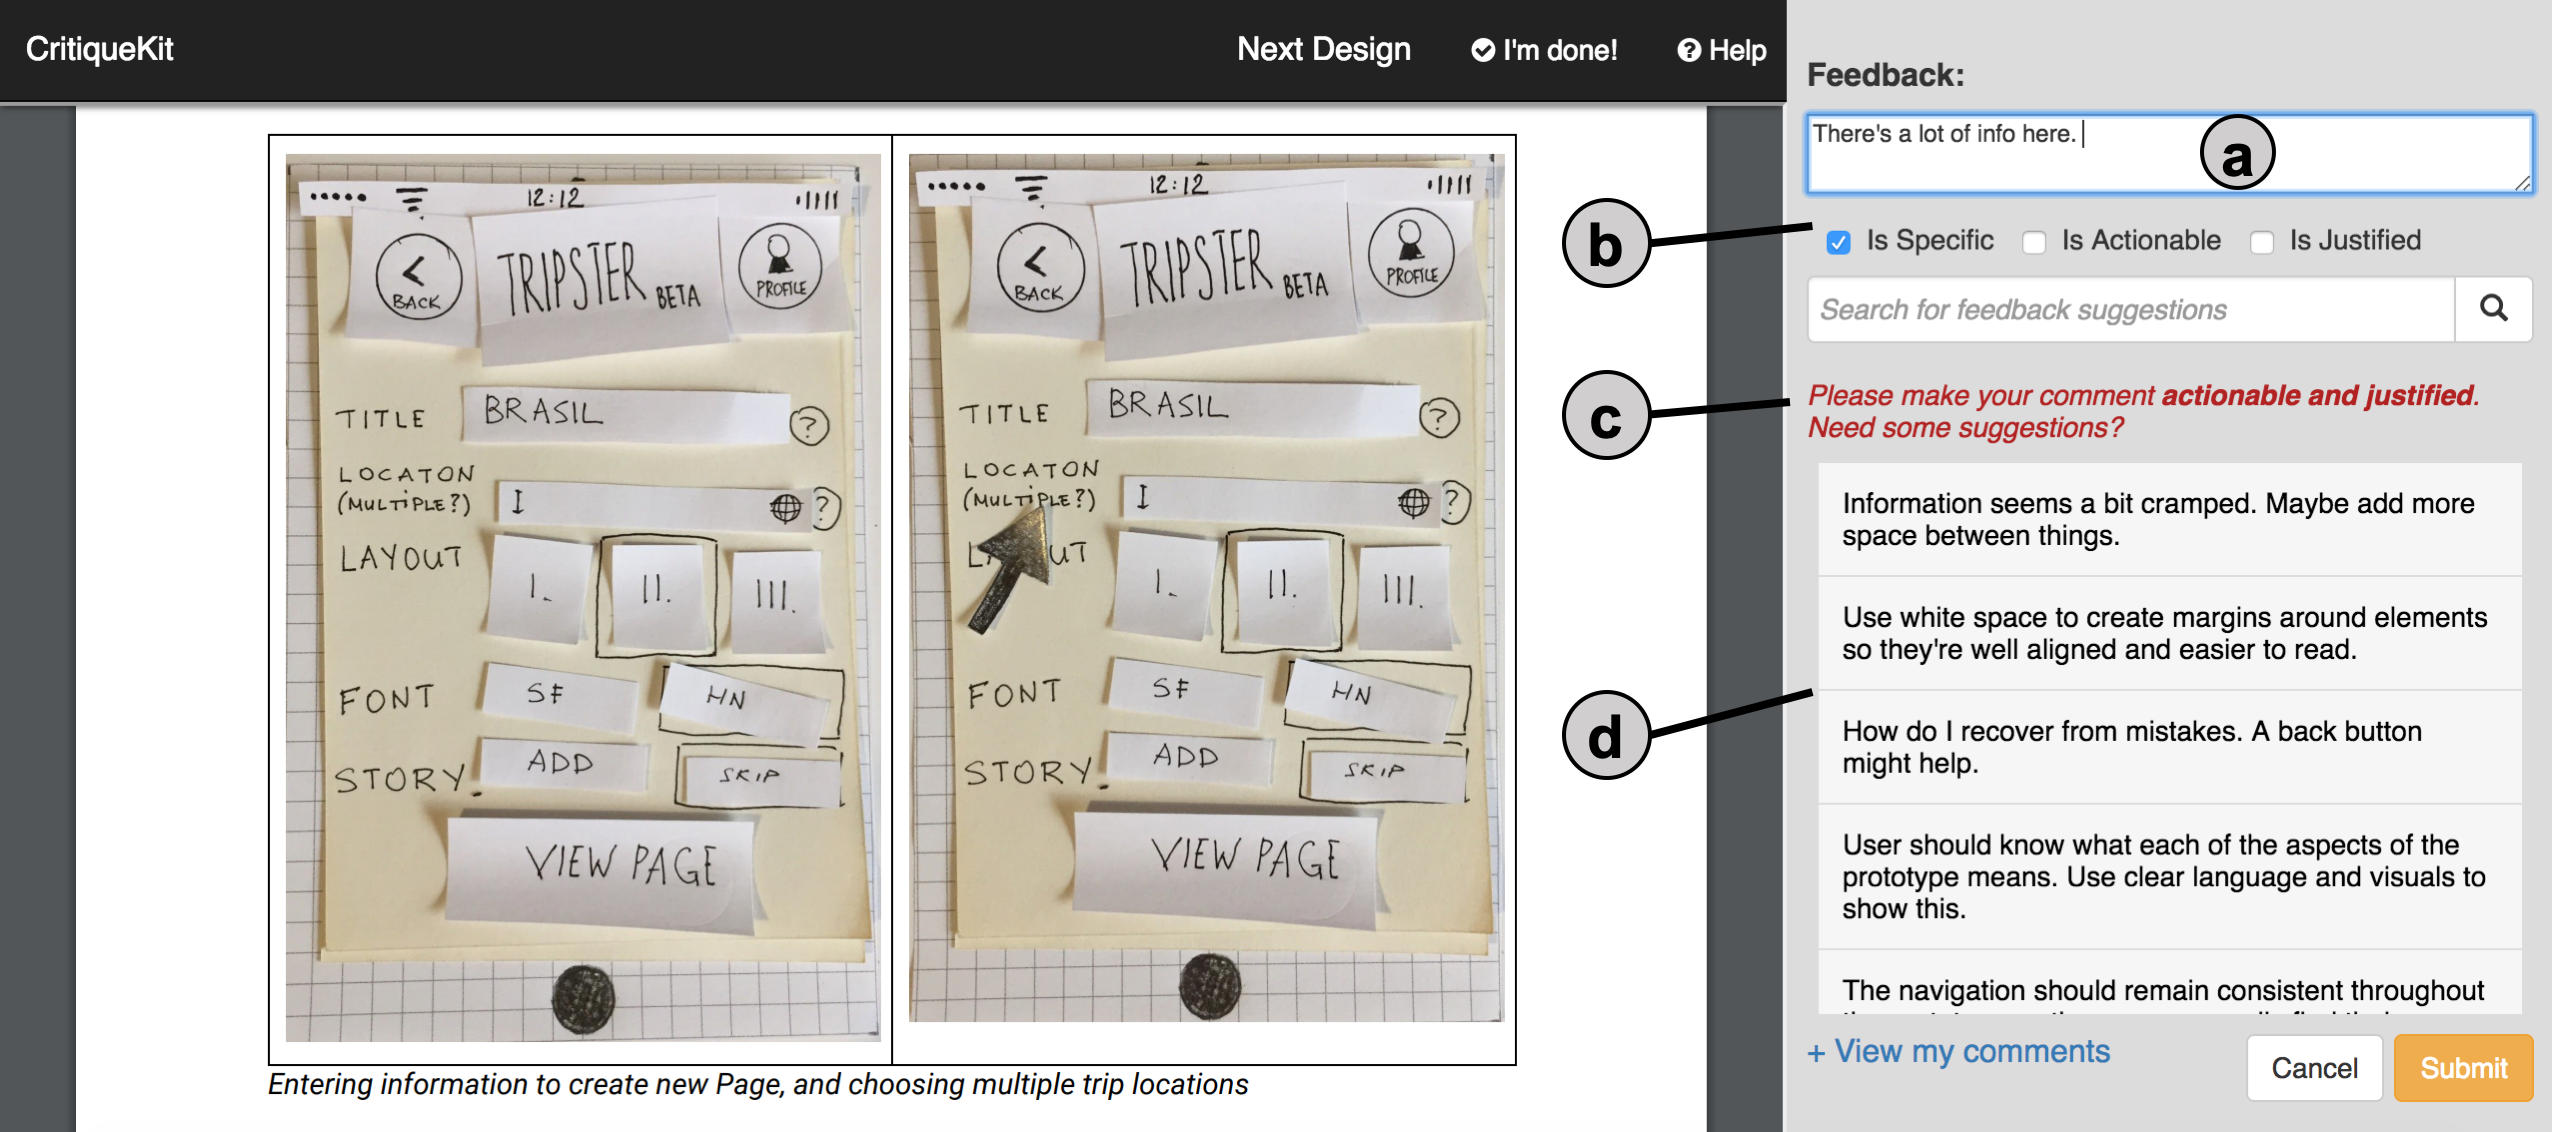
\includegraphics[width=\textwidth]{critiquekit/figures/interface.png}
  \caption[The final CritiqueKit interface for EXP 2.]{The final CritiqueKit interface for EXP 2. a) The reviewer can type their feedback in the textbox. b) The checkboxes in the guidance panel update based on the characteristics of the reviewer’s comments. c) CritiqueKit explicitly prompts reviewers to ensure their comment fits the checkboxes in the guidance panel. d) The reusable feedback suggestions in the suggestions box update based on the unchecked characteristics in the guidance panel, adapting the suggestions specifically to the reviewer's feedback.}~\label{fig:critiquekit_interface}
\end{figure}

\subsection{Interactive Guidance as a Form of Scaffolding}
CritiqueKit features an interactive guidance panel (\autoref{fig:critiquekit_interface}b) with checkboxes that update based on which of three attribute categories the feedback fits: \textit{Is Specific} \cite{Krause2017, Sadler1989, Sommers1982, Yuan2016}, \textit{Is Actionable} \cite{Dow2012, Gibbs, Kulkarni2015, Luther2015, Sadler1989, Tseng2007}, and \textit{Is Justified} \cite{Gielen2010, Krause2017, Narciss2006, Yuan2016}. 

The prototype assesses the feedback's fit with the following heuristics. The heuristic for the \textit{specific} category merely requires that comments be at least five words long because vague comments tend to be short, such as ``good job'' or ``needs work.'' Perhaps surprisingly, we observed that the five-word nudge was sufficient to garner specific feedback in practice. (Some websites, like Etsy, also use a five-word minimum heuristic for reviews). For the \textit{actionable} and \textit{justified} categories, we manually combed feedback that had been hand-labeled as meeting these categories and observed that specific keywords (i.e., ``maybe try'' and ``you should'' for actionable; ``because'' and ``so that'' for justified) were strong cues of these features. Consequently, the prototype implementation simply checks for the presence of these keywords and phrases in feedback comments. 

A comment is considered complete once all checkboxes are checked. Reviewers can manually check and uncheck the checkboxes if they feel the checkboxes did or did not add a category in error. For example, if a reviewer's comment states, ``Use a 2-column grid layout,'' and the ``Is Actionable'' checkbox remains unchecked, the reviewer can manually check the checkbox to note that their comment does indeed contain an actionable suggestion. 

\subsection{Adaptive Suggestions for Greater Specificity}
The suggestions box (\autoref{fig:critiquekit_interface}d) contains a list of previously given feedback from experts. These suggestions dynamically adapt based on how the reviewer's feedback is categorized in the guidance panel. For example, if a reviewer's comment does not yet satisfy the actionable and justified categories (as in \autoref{fig:critiquekit_interface}), the suggestions box would contain examples of feedback with these characteristics. Suggestions appear in the order they were added to the corpus.

\subsection{The CritiqueKit Review Workflow}
When a reviewer first opens CritiqueKit, a prompt asks them to provide specific feedback on something they like about the design and something that could be improved. The suggestions box contains general feedback snippets \cite{Kulkarni2013} pertinent to the review criteria to give reviewers a starting point, providing suggestions that are broadly applicable and fit within the specified criteria. The ``Submit'' button at the bottom of the interface is red to indicate that the comment text box is either empty or does not fit any of the categories in the guidance panel. 

Once a comment is sufficiently long, the ``Is Specific'' checkbox will check, and the reviewer will be prompted to make their comment actionable and justified. The ``Submit'' button turns yellow to indicate that their feedback is not yet complete, though they can still submit if desired. The feedback suggestions then change to present comments that instantiate both actionable and justified feedback. The suggestions continue to adapt depending on the characteristics of the comment, showing reusable examples of feedback that satisfy the unchecked categories in the guidance panel. Once all checkboxes are checked, the ``Submit'' button turns green as an indication of completeness. 

Using prior feedback as suggestions can give inspiration and highlight common issues. The presence of the structured guidance panel reminds reviewers of attributes that feedback should have. 

\subsection{Implementation}
CritiqueKit is a client-server web application implemented using Node.js; it assumes that all content to be reviewed is available on the web. The corpus of reusable feedback comments is stored on the server in JSON format.

CritiqueKit uses web sockets for communication between each client running the app and the main server, implemented using the socket.io module. Feedback classification happens on the client-side using JavaScript. Feedback suggestions are also generated on the client-side after retrieving the corpus from the server; the suggestions box adaptively shows and hides comments using JavaScript. 

Users access CritiqueKit by navigating to its URL in a web browser. The first time the browser loads the website, a unique ID is generated for the user and sent to the server. A cookie is also saved on the client-side so that the server can identify and differentiate users. The review content is loaded within the page as an iframe.

\section{Deployments: (How) Is Feedback Reused?}
To understand how feedback is reused in educational settings and evaluate the CritiqueKit approach, we conducted two deployments and two experiments. All studies took place at a research university. 

\subsection{DEP 1: How Do Teaching Assistants Reuse Feedback?}
Eight teaching assistants (TAs) (two female) for an undergraduate design course used Gradescope to grade and critique seven weekly assignments that varied in content from storyboards to written explanations to high-fidelity web application prototypes. TAs set rubric items for each assignment and wrote comments for each. We deployed CritiqueKit to first understand how TAs might reuse feedback and made iterative improvements to the design throughout the quarter based on TA input.

\begin{figure}[b!]
\centering
  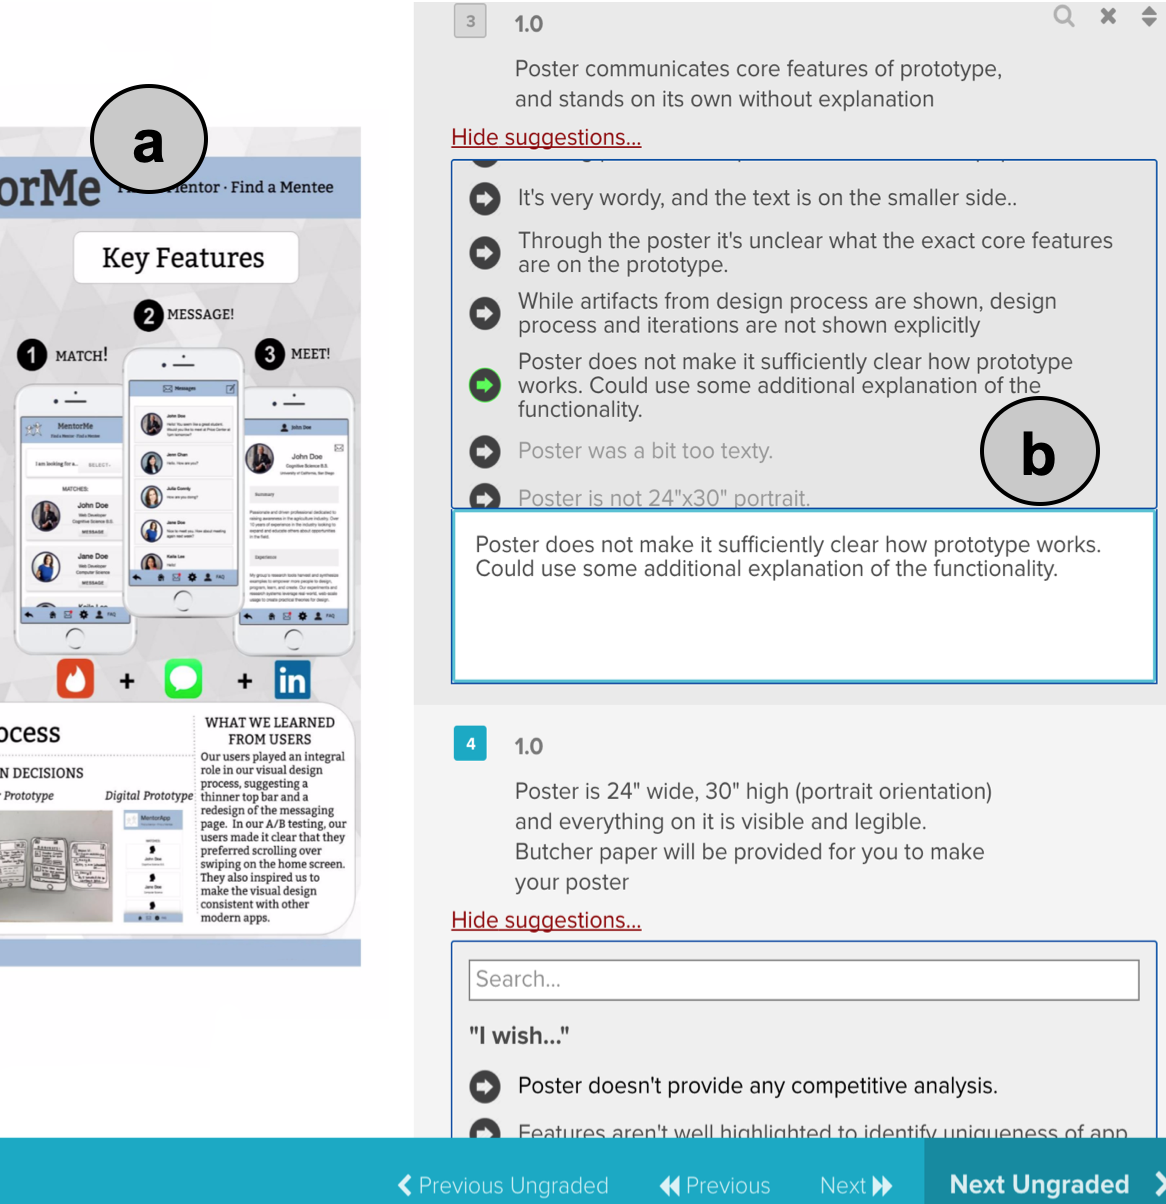
\includegraphics[width=0.6\textwidth]{critiquekit/figures/gradescope.png}
  \caption{CritiqueKit implemented as a browser extension in Gradescope for DEP 1. a) Reviewers provide feedback on a student design. b) The suggestions box under each rubric item provides reviewers with a list of reusable suggestions and a comment box for providing feedback on a submission.}~\label{fig:critiquekit_gradescope}
\end{figure}

\subsubsection{Method: Integrating CritiqueKit with Gradescope}
To integrate with the TAs' existing workflow, we implemented CritiqueKit as a Google Chrome extension that augments the Gradescope interface with a suggestions box (\autoref{fig:critiquekit_gradescope}). This version of CritiqueKit contained only the suggestions box to explore feedback reuse. The suggestions box contained a manually curated set of feedback provided by former TAs in a previous iteration of the course, stored in a Google Sheet online and retrieved by the Chrome extension using the Google Sheets API. Suggestions were categorized into three feedback categories: Positive, Problem, and Solution. TAs could select feedback suggestions to directly copy into the textbox for further editing. Each rubric item contained its own suggestion box interface, providing suggestions specific to that rubric item.

We curated the reusable suggestions corpus as follows. Given all feedback from the previous quarter, feedback that was 25 or fewer words in length was kept, because longer feedback was both too long to be skimmed in a suggestion display and tended to be overly specific. Feedback of 26-30 words was truncated at the sentence level to fit within the 25-word limit. Longer comments or duplicate comments were discarded. In total, 526 comments were provided as suggestions throughout the course for seven (of ten) assignments. Suggestions were manually categorized into the Positive ($n = 92$), Problem ($n = 312$), and Solution ($n = 122$) categories.

\subsubsection{Result: TAs Used Feedback Suggestions as Inspiration}
Across seven assignments, four of the eight TAs reused 51 distinct suggestions from the 526-element corpus (9.7\%). 75 of 583 designs received a reused suggestion for feedback. 60\% of reused suggestions were categorized in the Problem category. These numbers omit any reuse occurring entirely inside Gradescope without CritiqueKit. (Gradescope provides an interface for reusing entire comments within an assignment rather than for individual parts of the comment.) 

An end-of-course survey asked TAs about their CritiqueKit use. One commented that he would ``\textit{skim the comments in the [suggestions] to see if something was accurate to my thoughts}.'' Another mentioned that the prototype helped him ``\textit{[find] ways to better explain and give feedback about specific points}.'' TAs also mentioned that suggestions sometimes reminded them to comment on more diverse aspects of students' work. For example, one mentioned that seeing positive suggestions reminded her to give positive feedback, not only critiquing areas for improvement. TAs mentioned using the suggestions as inspiration rather than the exact wording, taking the underlying concept of a suggestion and tailoring it.

\subsection{DEP 2: How Do Students Reuse Feedback?}
The first deployment examined teaching staff usage; this second deployment examined student usage to understand how novices interact with guidance and suggestions. We deployed CritiqueKit as a standalone web application with 29 students in an undergraduate design course for five weeks. Students gave anonymous feedback on two randomly assigned peer submissions for each of seven assignments.

\begin{figure}[b!]
\centering
  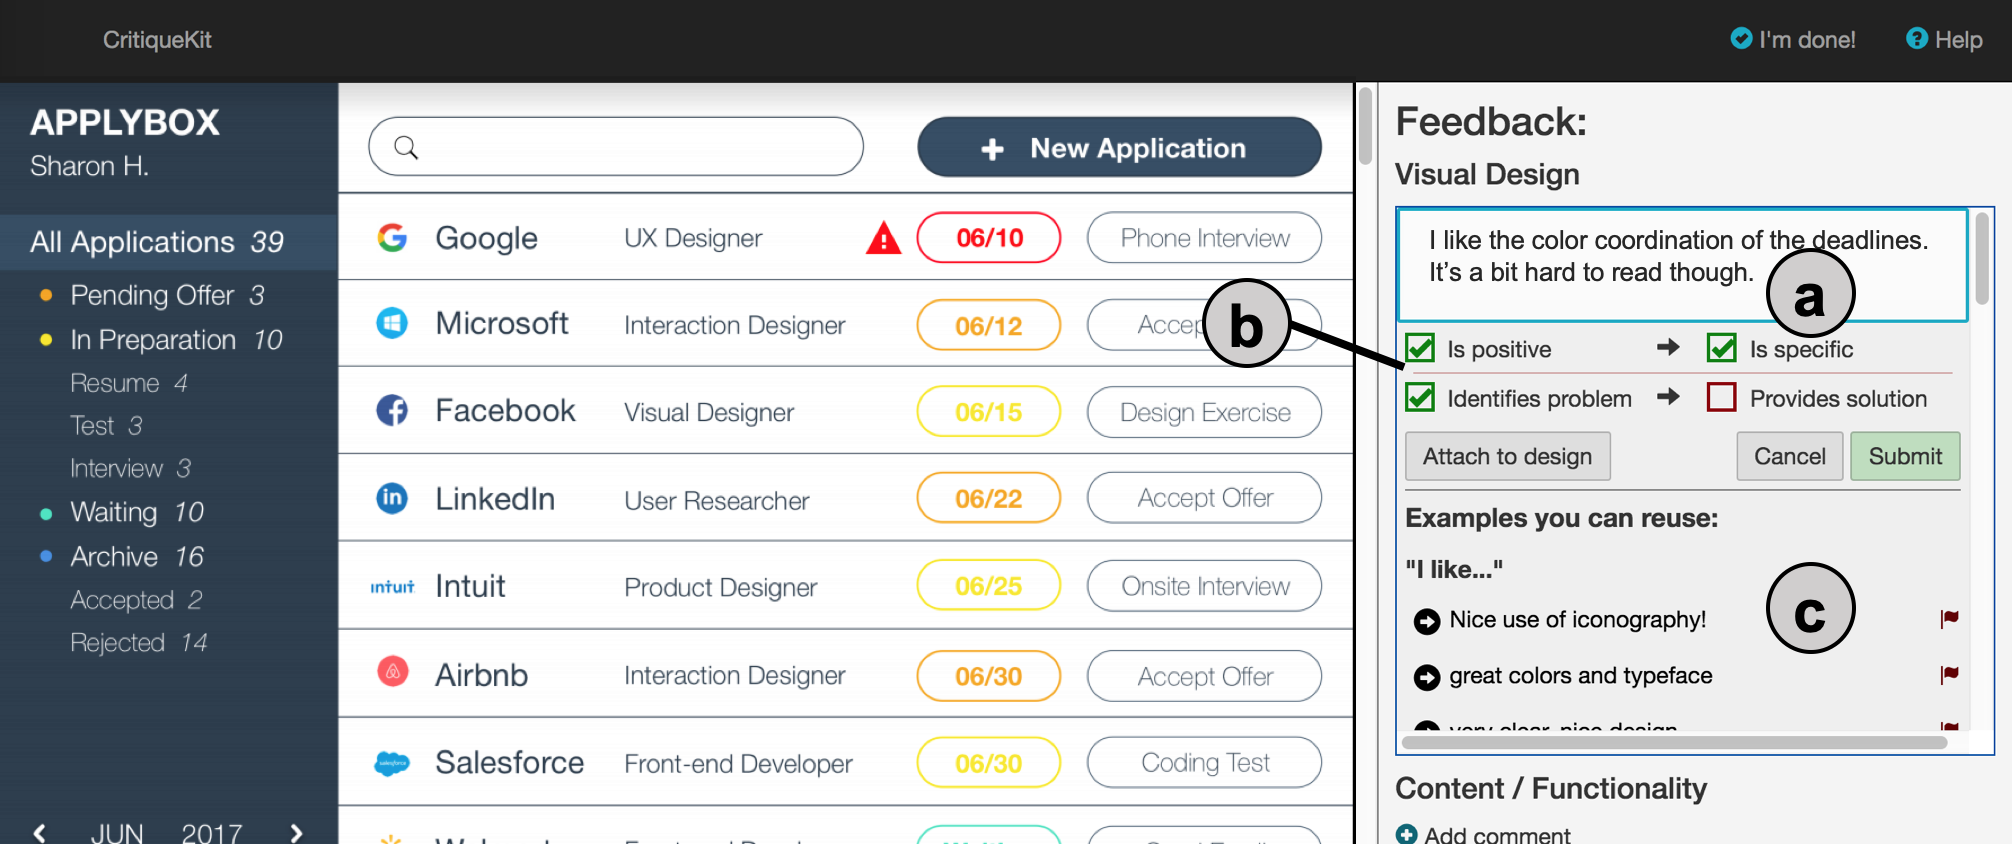
\includegraphics[width=\textwidth]{critiquekit/figures/old_interface.png}
  \caption[The CritiqueKit user interface for DEP 2 and EXP 1.]{The CritiqueKit user interface for DEP 2 and EXP 1. a) The reviewer types their feedback into the text box. b) Checkboxes in the guidance panel update as the reviewer types to show how well the comment fulfills high-quality feedback criteria. c) The reviewer can browse and reuse previously given feedback.}~\label{fig:critiquekit_exp1}
\end{figure}

\subsubsection{Method: Integrating Interactive Guidance for Scaffolding}
Novice students are less experienced in giving feedback and may benefit from interactive scaffolding \cite{Reiser2004}. This version of CritiqueKit included an interactive guidance panel to help reviewers provide more specific and actionable feedback (\autoref{fig:critiquekit_exp1}). The categories on the guidance panel were ``Is Positive,'' ``Is Specific,'' ``Identifies a Problem,'' and ``Presents a Solution'' with checkboxes next to each. These categories stem from recommendations in the literature for both positive and critical feedback \cite{Kelley2013}. Similar to the final version of CritiqueKit, these checkboxes updated as a reviewer typed by classifying their comment into the three categories. The categories differed from the final version, focusing on specific and actionable feedback. 

The suggestions box was seeded with feedback from the course TA. Similar to the first deployment, the suggestions were categorized in the Positive, Problem, and Solution categories. When a student submitted a comment, it was classified into one of these categories, shortened to 25 words if it was longer, and fed back into the corpus to appear as a suggestion, enabling students to reuse their peers' as well as their own comments. The suggestions were ordered first by frequency used, then by shortest length first, and updated as these values changed and more comments were added. Compared to the final version of CritiqueKit, suggestions were static, meaning they did not change as the reviewer typed.

\subsubsection{Results: Positive Feedback Common; Reuse Rare}
For seven assignments, 898 comments were submitted. Independent raters classified each comment into the five categories of Positive Only, Positive  and  Specific (Positive + Specific), Problem Only, Solution Only, and Problem with a Solution (Problem + Solution). 45\% of these comments contained positive feedback; 30\% contained a Problem + Solution statement. 

Students rarely selected feedback suggestions for reuse. Over the five-week deployment, 14 distinct suggestions were reused on 27 student designs for four of the seven assignments. These suggestions were mostly short, vague comments such as ``I wish this was more visually appealing.'' This may be because students often left feedback specific to individual designs that did not easily generalize to other contexts. Students' comments in a post-survey confirmed that the suggestions did not always seem applicable. Students also did not regularly use the interactive guidance panel; 15 of the 29 students engaged with the panel a total of 120 times over five weeks. 

In contrast to how TAs reused feedback, students may not have recognized common issues. TAs paid attention to common errors between designs and mainly reused Problem feedback, whereas students may not have noticed or attended to underlying issues between designs. For instance, one student mentioned that they did not use the feedback suggestions because they ``\textit{rarely pointed out the same things when critiquing interfaces}.'' 

This exploratory deployment investigated how students reuse feedback and respond to interactive guidance in the classroom. To understand how a system with these features compares to a standard feedback system, the next study was a controlled between-subjects experiment. 

\section{Experiments: Scaffolding Feedback}
Following our deployments, we conducted two empirical studies to investigate the impact of suggestions and guidance on feedback quality.

\subsection{EXP 1: Do Static Suggestions Improve Feedback?}
In an online between-subjects study, 40 undergraduate design students were asked to review three restaurant website homepages using CritiqueKit. The task emulated peer review tasks often required in creative courses. This study's suggestion corpus came from a design feedback task on CrowdCrit \cite{Luther2015} and was categorized in the Positive, Problem, and Solution categories. We hypothesized that suggestions and guidance would help reviewers provide more specific and actionable comments.

\subsubsection{Method: Reviewing Restaurant Websites}
40 participants were randomly assigned to either the CritiqueKit condition or the Control condition (20 in each). CritiqueKit participants used the same version of CritiqueKit as DEP 2 with all features available (\autoref{fig:critiquekit_exp1}). Control participants used an otherwise identical version consisting solely of a comment text box. Upon landing on the homepage of either version, participants were provided with a scenario explaining that three restaurant owners are seeking feedback on their new website design. Participants were given a brief tutorial of CritiqueKit's features and an explanation of what makes for good feedback. There were no restrictions or requirements on time spent or amount of feedback to provide. We compared the percentages of comments in five categories. Comments including a supportive element were labeled as \textit{Positive Only} or \textit{Positive + Specific}. Comments including a critical element were labeled \textit{Problem Only}, \textit{Solution Only}, or \textit{Problem + Solution}.

\begin{figure}[b!]
\centering
  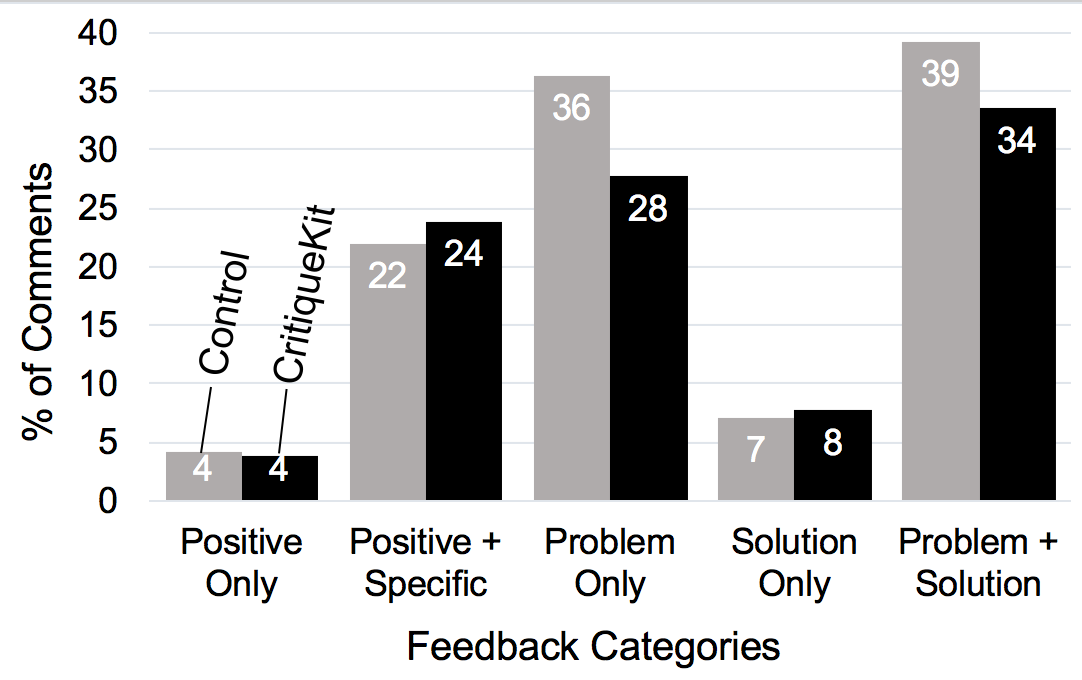
\includegraphics[width=0.6\textwidth]{critiquekit/figures/exp1_feedbacktypes.png}
  \caption{A plurality of feedback in both conditions in EXP 1 identified both a problem and solution (\textit{i.e.}, was actionable). Feedback that was only positive was the rarest. There were no significant differences between conditions for these categories.}~\label{fig:critiquekit_exp1_results}
\end{figure}

\subsubsection{Results: Static Suggestions Were Not Helpful}
With static suggestions and interactive guidance, there were no significant differences between conditions. (To foreshadow, we will see differences in EXP 2, which adds adaptive suggestions). Participants provided a total of 323 comments (168 for control, 155 for CritiqueKit). The average number of words per comment was not significantly different between conditions (Control: $m = 29.07, SD = 23.64$; CritiqueKit: $m = 23.22, SD = 17.3$) ($F(1,38) = 2.52, p = .11$).

\subsubsection{Suggestions \& Guidance Did Not Affect Type of Feedback}
The distribution of the five category types did not vary significantly between conditions ($x^2 = 4.80, df = 4, p = .31$) (\autoref{fig:critiquekit_exp1_results}). In both groups, participants provided mostly Problem + Solution feedback (39\% in Control; 34\% in CritiqueKit). 

\subsubsection{Most CritiqueKit Participants Corrected Category Labels}
65\% of CritiqueKit participants actively used the guidance panel, making a total of 85 corrections to categories. Interaction with the guidance panel may have indicated attention to the feedback characteristics. As the study was online, we don't know how many of the other 35\% were influenced by the guidance panel. 

\subsubsection{Unfortunately, People also Reused Vague Suggestions}
11 distinct suggestions from the corpus were reused. 8 of these were vague; 3 were specific. 15 of 155 reviews included a reused suggestion. This seems especially low given the high engagement with the guidance panel. We see two reasons for this: First, the suggestions came from CrowdCrit \cite{Luther2015}, where participants provided feedback on a weather app design. The study task was different than the task for which the suggested feedback was originally given, and novices may have had a limited ability to see the deep structure behind a suggestion and reapply it in a new context. Second, the suggestions were created by crowd workers and of uneven quality. 

The suggestions selected were typically short, positive comments, perhaps because students did not know how to apply them in the specific context. For example, the most commonly reused suggestion was ``great use of color'' (reused 3 times). This result is similar to DEP2 in which students did not find feedback provided by other peers or novices to be useful and generalizable. Feedback suggestions may require more curation or quality control to be most useful. 

\subsubsection{Suggestions \& Guidance Should Work in Concert}
While this version of CritiqueKit contained both feedback suggestions and interactive guidance, these features functioned independently. Regardless of the categories checked in the guidance panel, the suggestions remained static and presented in the same order for each participant, potentially making them easy to ignore if they were irrelevant to the context. Participants may have paid attention to only one feature at a time. The next study investigated the question of whether adaptively presenting feedback suggestions along with interactive guidance improves feedback. 

\subsection{EXP 2: Do Adaptive Suggestions Help?}
The second experiment used the final version of CritiqueKit described in the system section to test the hypothesis that adaptively-presented suggestions combined with guidance would improve feedback by increasing the fraction of feedback that is specific, actionable, and/or justified.

\subsubsection{Method: Reviewing Paper Prototypes}
We conducted a between-subjects in-person study with 47 (27 female) participants. Participants were recruited from an undergraduate subject pool within the Psychology and Cognitive Science departments. Participants were randomly assigned to either the CritiqueKit ($n = 24$) or Control ($n = 23$) conditions. 44 of these participants had no design course experience; 3 participants had taken at least one design course. 28 spoke English as a second language. 

Participants were asked to provide feedback on two designs from students enrolled in an online course who volunteered to receive more feedback on their work. These designs were PDFs of mobile application paper prototypes. The review criteria included whether the prototype supported the student's point of view and whether it seemed easily navigable. Participants were first shown the design instructions and review criteria and then given a short tutorial of CritiqueKit as well as an explanation of what makes for good feedback. CritiqueKit participants had all features of CritiqueKit available to them (\autoref{fig:critiquekit_interface}), while Control participants used a version that consisted of only a textbox for their feedback. The task took about 30 minutes to complete. After providing feedback on both designs, participants were interviewed about their feedback process and use of CritiqueKit. 

\subsubsection{Presenting Feedback Suggestions Adaptively}
The categories on the guidance panel and their definition used for coding participants' responses were the following:\\
\textbf{Specific}: relates directly to the review criteria\\
\textbf{Actionable}: gives a concrete suggestion for improvement\\
\textbf{Justified}: provides a reason for why something is done well or should be improved

For DEP 2 and EXP 1, the guidance panel categories sought to encourage specific and actionable feedback (\autoref{fig:critiquekit_exp1}). Examining the feedback from our previous studies, we found that ``Is Positive'' and ``Identifies a Problem'' did not provide significant guidance as reviewers were generally aware of whether their feedback was positive or critical. In addition, the guidance panel did not explicitly check for justification of feedback. For EXP 2, we revised the categories to ``Is Specific,'' ``Is Actionable,'' and ``Is Justified'' to also encourage the explanation or reasoning behind feedback. As described in the system section, the checkboxes update as the reviewer types to reflect the categories present in their comment, and the suggestions adapt to show feedback examples from categories not yet present in the comment. 

\subsubsection{Results: CritiqueKit Participants Provided More Specific, Actionable, \& Justified Feedback}
Participants provided 158 total comments (79 control, 79 CritiqueKit). The percentage of comments that contained all three categories (specific, actionable, and justified) was significantly higher in the CritiqueKit condition (53\%) than in Control (30\%) ($x^2=8.33, df = 1, p = .01$) (\autoref{fig:critiquekit_exp2}). As an example, this comment meets all three: ``The `more questionnaires' section (Specific) should be made smaller (Actionable) because it is not the main focus of the page.'' (Justified). The system's heuristic for checking specificity of a comment was quite simple: five words or greater in length. Feedback raters blind to each condition used a more sophisticated and holistic assessment, taking specific to also mean related to the review criteria. With this assessment, 98\% of CritiqueKit comments were labeled by raters as specific whereas only 83\% of Control comments were. These raters also rated comments from EXP 1 within the specific, actionable, and justified categories to provide a comparison between the two experiments. Interestingly, the percentage of comments containing all attributes in the Control condition was relatively consistent between EXP 1 (35\%) and EXP 2 (30\%). The percentage of comments with all attributes in the CritiqueKit condition greatly increased between the two experiments (26\% versus 53\%). Having the checkboxes may have explicitly reminded CritiqueKit participants to ensure their comments satisfy the specific, actionable, and justified categories.

\begin{figure}[b!]
\centering
  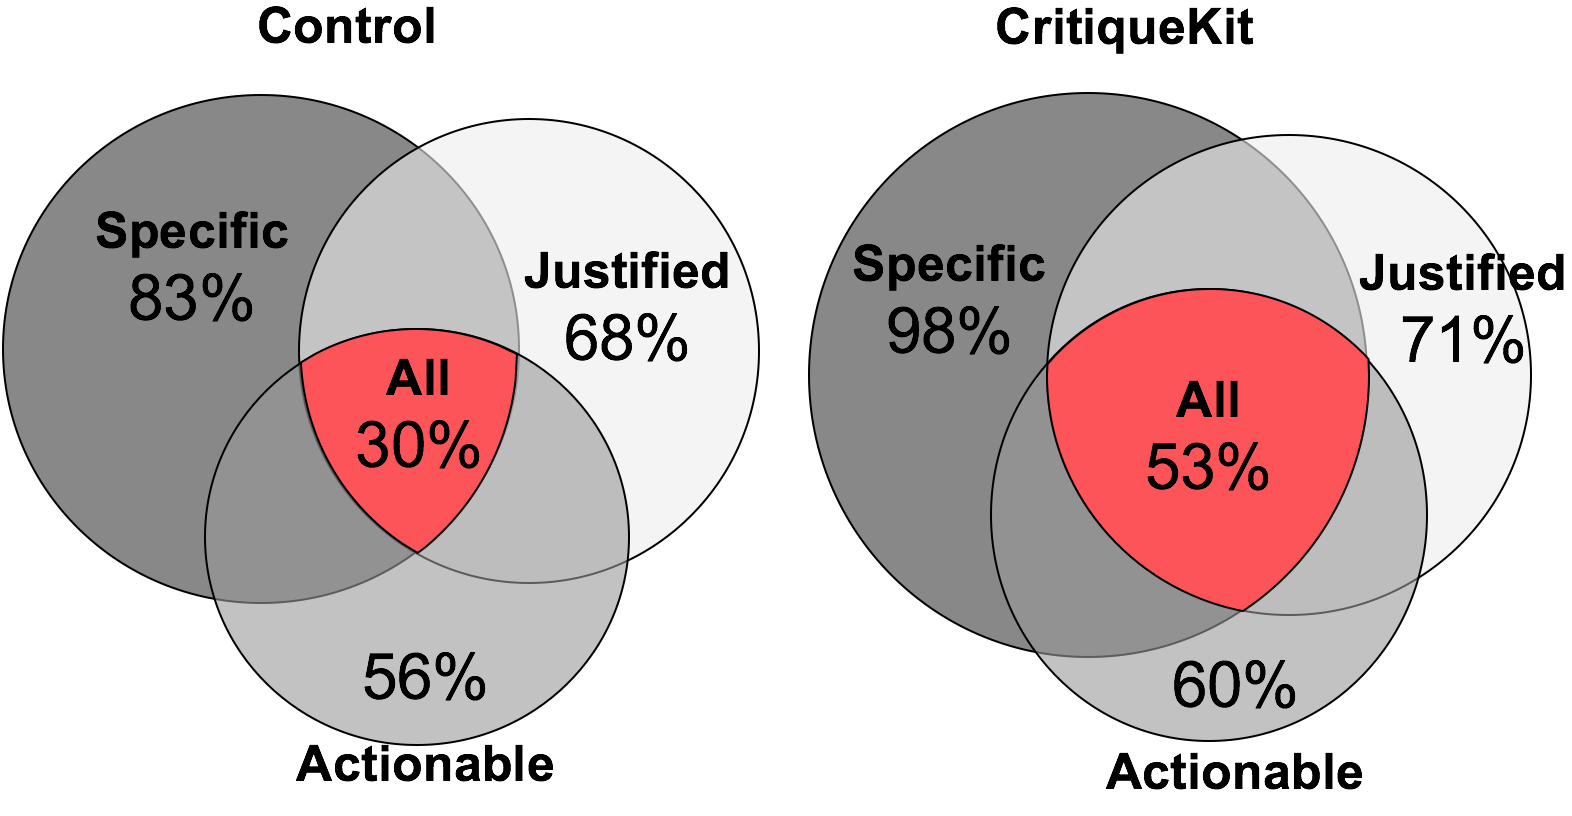
\includegraphics[width=0.6\textwidth]{critiquekit/figures/venn_diagram_exp2.png}
  \caption{In EXP 2, a significantly higher percentage of feedback in the CritiqueKit condition (53\% versus 30\%) contained three attributes of good feedback: Specific, Actionable, and Justified.}~\label{fig:critiquekit_exp2}
\end{figure}

\begin{figure}[b!]
\centering
  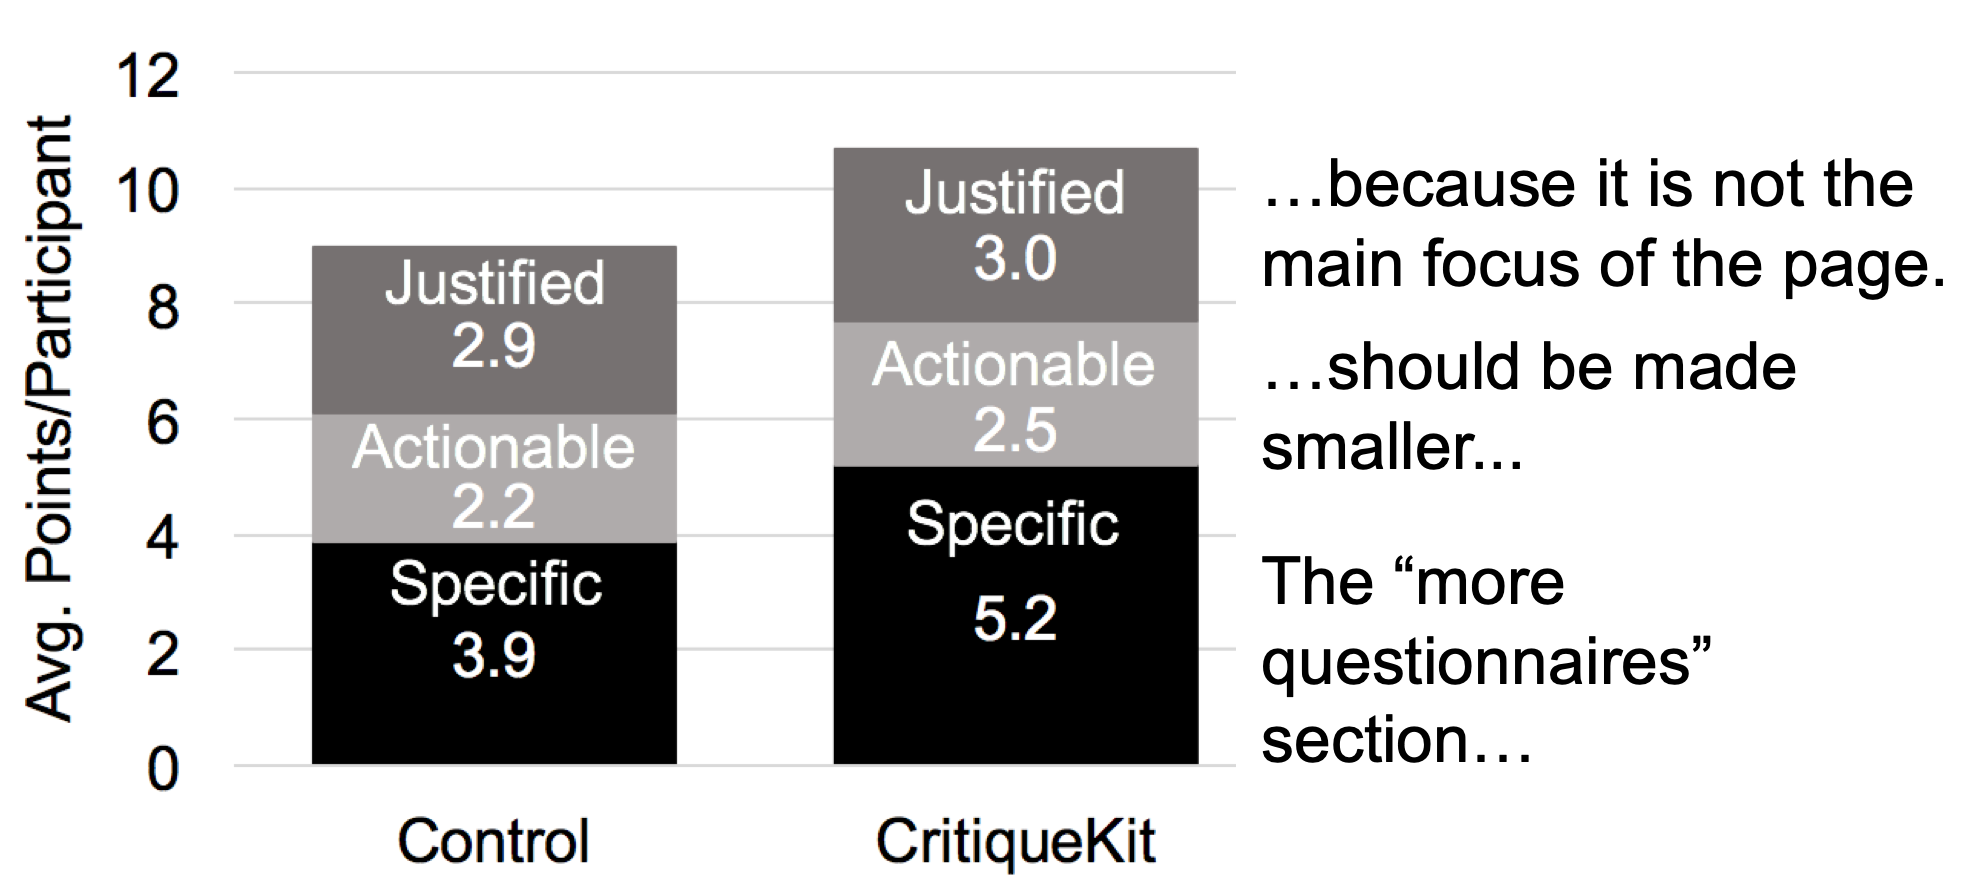
\includegraphics[width=0.6\textwidth]{critiquekit/figures/exp2_bar.png}
  \caption{CritiqueKit participants provided more \textit{specific} and \textit{all-three} category ideas than control participants.}~\label{fig:critiquekit_exp2_bar}
\end{figure}

Because longer comments were more likely to contain all three categories, each comment was also scored on a point scale and averaged per participant. Comments received one point for each specific, actionable, and justified idea (\autoref{fig:critiquekit_exp2_bar}). A \textsc{manova} with category points as dependent variables shows a significant difference between conditions ($F(1,3) = 3.21, p < .005$). CritiqueKit participants provided more specific ideas than Control participants (Control $m = 3.87$, CritiqueKit $m = 5.17$, $F(1,156) = 14.04, p  <  .05$). This may be because the suggestions provided examples of relevant ideas and led CritiqueKit participants to address more. CritiqueKit participants also provided more ideas that fit all three categories than control (Control $m = 1.0$, CritiqueKit $m = 2.2$, $F(1,156) = 8.78, p < .005$). Given that most participants did not have any design experience, the combination of adaptive suggestions and guidance may have been most useful for these reviewers. The suggestions may have provided a starting point while the guidance panel helped them understand how to apply the attributes of good feedback. There were no significant differences in the average number of actionable and justified ideas in comments.

On average, Control comments were 39.3 ($SD = 30.3$) words long and 43.7 ($SD = 31.4$) words for CritiqueKit comments. There was no significant difference in comment length ($F(1,156) = 1.77, p = .19$). Unfortunately, we don't know how the feedback improved students' work because they received feedback from both Control and CritiqueKit participants. A longitudinal deployment with the final version of CritiqueKit would likely be more useful in determining the helpfulness of feedback.

\subsubsection{Suggestions Helped Reviewers Describe Their Thoughts}
Participants rated the suggestions as being generally helpful ($m = 4.29, SD = 0.95$, 1-5 Likert Scale). When asked to elaborate on their rating, many participants noted that the suggestions helped them describe their thoughts. One participant remarked, ``\textit{I was a bit lost at first because I didn't know how to describe my thoughts. The suggestions helped me figure out how I should describe what I was thinking}.'' Similarly, another mentioned that ``\textit{when I [didn't] know how to put my feedback in words, I could look at the suggestions}.'' Particularly for participants without any design experience, suggestions helped with appropriate language to use in their feedback. For example, one noted that ``\textit{seeing actual wording from a designer's point of view was good so you know how to say what you want to say}.'' Though a few participants did not directly select suggestions, it is likely that they were inspired or influenced by them as they used similar wording in their own comments. 

Still, some participants felt the suggestions were too general and not entirely relevant to the specific design they were reviewing. One participant felt constrained by the suggestions, stating that she ignored them because she wanted to write her own opinions. Suggestions seemed most helpful for participants who used them as a starting point for their own thoughts rather than solely relying on them. Participants who simply selected suggestions tended to list issues without adding their own elaboration. This behavior not only led to incomplete feedback, but also produced depersonalized and scattered comments. For example, one comment that solely relied on suggestions reads ``User immediately knows the purpose of the prototype. Good use of grid layout to keep items aligned. Icons should be immediately recognizable to the user.'' A consideration for future work is to develop feedback suggestions tailored to help reviewers provide more cohesive and contextual comments. 

Most participants in this experiment did not have any design experience and may have benefited most from the suggestions. Many participants noted using the suggestions as a way to find ideas whereas students with design experience may already have heuristics and processes in mind when providing feedback. Future work should examine how suggestions and guidance might improve feedback for more experienced learners as well.

\subsubsection{Interactive Guidance Helped Remind \& Focus Reviewers} 
Participants were mixed on the helpfulness of the guidance panel ($m = 3.67, SD = 1.2$, 1-5 Likert Scale). Those who did find it helpful noted that the categories helped guide their feedback process. For instance, one participant noted that he ``\textit{went in order of the checkboxes. First, I provided something specific, then something actionable, then justified it}.'' Another noted that the categories helped her know whether her feedback was actually useful or helpful, and one noted that the guidance panel ``\textit{[made] sure the feedback is complete and not vague}.'' 

Anecdotally, we observed that when participants said the categories were not useful, it was because they believed them to be inaccurate in their classifications. The accuracy (compared to human raters) for the actionable category was 67\% and 75\% for the justified category. A participant stated that ``\textit{[the checkboxes] didn't always check when I thought they should, so I would just do it myself}.'' Another thought the checkboxes were ``\textit{quick to judge, it felt like it wasn't reading what I was saying}.'' Three participants, who were not native English speakers, found the categories confusing because they weren't sure what they meant. Future iterations of CritiqueKit could include the definition of these categories in the prompts to make the meaning clearer. Interestingly, a couple participants noted that they used the categories as reminders rather than for active guidance. For instance, a participant mentioned that though he felt the interactive guidance was not that accurate, ``\textit{[the checkboxes] reminded me to make sure my comment contained specific, actionable, and justified parts, so I'd go and reread through my comment}.'' 

Some participants commented on the adaptive presentation of the suggestions with the guidance panel. For one participant, the suggestions helped him understand what the categories meant. He noted, ``\textit{The whole actionable and justified thing, I didn't know what that meant, so the suggestions helped with that}.'' Observations of participants showed that some clicked on the checkboxes simply to see the suggestions under each one. When asked about how useful they found CritiqueKit in general, participants varied widely in their ratings of usefulness. A more precise measure would allow participants to compare across conditions, which was not possible with this between-subjects design. 

\section{General Discussion}
This chapter empirically investigated two techniques for scaffolding feedback: reusable feedback suggestions and adaptive guidance. This work complements this dissertation more broadly, highlighting the benefits of adaptive guidance for interfaces that support creative tasks. Here we discuss and synthesize the findings.  

\subsection{Generating Reusable Feedback Suggestions}
This work investigated whether suggestions and guidance can scaffold the feedback process. For this strategy to work, an eye towards reuse and adaptive feedback must be adopted. As Schön argues, experts may be most capable of recognizing common patterns and giving useful feedback \cite{Schon1983}. However, while feedback should be specific, underlying concepts can generalize across contexts. In the studies that used expert-generated feedback suggestions (DEP 1 and EXP 2), participants cited the same reason for why the suggestions were useful: as inspiration. Participants reported that the suggestions helped them find words for their thoughts or helped direct their attention to issues they did not originally notice. This suggests that reusable suggestions should focus attention to common issues rather than specific instances. Our approach demonstrates how expertise on creative work can be scaled by providing feedback on a few to apply to many \cite{Kulkarni2013}. This extends work on reusable feedback in coding and writing \cite{Brooks2014, Hartmann2010, Head2017} while keeping the human in the loop, enabling novices to learn and reuse expert insights. 

It is possible that more general suggestions can lead to less personalized feedback, particularly in abstract domains like visual design. We observed this in 7 of the 79 comments from the CritiqueKit condition in EXP 2, in which the four participants simply selected suggestions without further elaboration. A consideration for creating and presenting reusable suggestions is how these suggestions can be both general yet personal to be more helpful to the recipient. 

\subsection{What is the Best Way to Guide Feedback?}
Prior empirical work on feedback (\textit{e.g.}, Kulkarni \textit{et al.} \cite{Kulkarni2013} and Krause \textit{et al.} \cite{Krause2017}) has not compared static and adaptive suggestions. In this chapter, we found that people rarely used static suggestions and did not find them helpful; adaptive suggestions were used more and found more helpful. This reinforces prior work demonstrating that adaptive presentation of examples can improve learning \cite{Lee2010, Najar2014}. By presenting feedback suggestions that directly addressed missing characteristics of a reviewer's feedback, reviewers were prompted on where they could specifically improve, and explicitly shown examples of how to do so. 

The second experiment adapted feedback suggestions based on whether their feedback was categorized as specific, actionable, and/or justified. Though some of the prototype's categorizations were misleading or inaccurate (for example, the comment ``user flow is simple'' was categorized as ``Is Actionable'' because of the word ``use'', even though it lacks a concrete suggestion), participants still referenced the three categories when composing their comments. The guidance panel was useful as a reminder to include the attributes of good feedback in their comments. A more sophisticated method for categorization would likely be helpful, though our naïve approach performed reasonably well overall.

The guidance panel focused on three important attributes of good feedback. A consideration is to also provide guidance for emotional content in feedback, as emotional regulation is important to how learners perceive feedback \cite{Krause2017, Varlander2008}. In addition, other characteristics may also contribute to perceived helpfulness, such as complexity or novelty \cite{Krause2017}, that could be further explored through adaptive guidance.

\subsection{Creating Adaptive Feedback Interfaces}
In order for adaptive guidance to be most effective, the interface should be suitable for adaptation. In the two deployments and first experiment, the suggestions were not curated in any way: more than 1,400 comments were supplied as suggestions, but only 76 of these were reused by reviewers. Having more suggestions available was not beneficial because the suggestions were not sufficiently adaptable and were potentially irrelevant and difficult to browse. EXP 2 introduced a curated approach: experts provided the suggestions with generalizability in mind. Of the 47 suggestions created, 29 were reused. Though fewer suggestions were available, they were more general and adaptable, potentially making them more useful. 

Suggestion presentation shares many properties with search interfaces. Like with search, a good result needs to not only be in the set, but toward the top of the set \cite{Hearst2009Book}. The second experiment contained fewer suggestions, enabling easier search and browsing. Effective curation and display of suggestions should take into consideration the quality of feedback suggestions and how likely they are to be selected, potentially using frequency or some measure of generalizability as a signal. 

\section{Conclusion}
Looking across the deployments and experiments, adaptive suggestions and interactive guidance significantly improved feedback while static suggestions did not offer significant improvements. These techniques were embodied in the CritiqueKit system, used by 95 feedback providers and 336 recipients. Future work should examine applying other attributes of helpful feedback and further investigate how best to create, curate, and display adaptive suggestions. 

Much knowledge work features both underlying principles and context-specific knowledge of when and how to apply these principles. Potentially applicable feedback and review areas include domains as disparate as hiring and employee reviews, code reviews, product reviews, and reviews of academic papers, screenplays, business plans, and any other domain that blends context-specific creative choices with common genre structures. We hope that creativity support tools of all stripes will find value in the ideas and results presented here.


\section{Acknowledgements}
We thank Kandarp Khandwala and Janet Johnson for help rating feedback. This research was supported in part by a fellowship from Adobe Research.

This chapter, in part, includes portions of material as it appears in \textit{Interactive Guidance Techniques for Improving Creative Feedback} by Tricia J. Ngoon, C. Ailie Fraser, Ariel S. Weingarten, Mira Dontcheva, and Scott Klemmer in the Proceedings of the 2018 CHI Conference on Human Factors in Computing Systems (CHI '18). The dissertation author was one of the primary investigators and authors of this paper.
